\documentclass[t,xcolor={usenames,dvipsnames}]{beamer}

\mode<presentation>
{
\usetheme{Frankfurt}%{Warsaw}
%\setbeamercovered{transparent}
%\setbeamercolor{background canvas}{bg=white}
}

% Delete these, if you do not want the table of contents to pop up at
% the beginning of each (sub)section:
%\AtBeginSubsection[]
%{
%  \begin{frame}<beamer>{Outline}
%    \tableofcontents[currentsection,currentsubsection]
%  \end{frame}
%}
%\AtBeginSection[]
%{
%  \begin{frame}<beamer>{Outline}
%    \tableofcontents[currentsection]
%  \end{frame}
%}

\usepackage[english]{babel}
\usepackage[latin1]{inputenc}
\usepackage{times}
\usepackage[T1]{fontenc}
\usepackage{verbatim}
\usepackage{url}
\usepackage{amsmath,amssymb}
\usepackage{comment}

% Author-date citations
\usepackage[authoryear,round]{natbib}
\let\cite=\citep  % default \cite such as {\LaTeX} authors are used to

% Where \includegraphics should look for figures
\graphicspath{{./figs/}}
\usepackage{epstopdf}
\DeclareGraphicsExtensions{.eps,.png,.jpg,.pdf}

% Shortcuts
\newcommand{\myhref}[2]{\href{#1}{\textcolor{Blue}{#2}}}
\newcommand{\subitem}[1]{\begin{itemize}\item #1 \end{itemize}}
\newcommand{\ghead}[1]{{\tiny #1\\}}

%%%%%%%%%%%%%%%%%%%%%%%%%%%%%%%%%%%%%%%%%%%%%%%%%%%%%%%%%%%%%%%%%%%%%%
\title{Functional Curation of Cardiac Cellular Models}
\author{Jonathan Cooper}
\institute[University of Oxford]
{Computational Biology Group\\
 Department of Computer Science\\
 University of Oxford}

\begin{document}

\begin{frame}
\titlepage
\end{frame}

%%%%%%%%%%%%%%%%%%%%%%%%%%%%%%%%%%%%%%%%%%%%%%%%%%%%%%%%%%%%%%%%%%%%%%

\begin{frame}{Outline}
\tableofcontents
\end{frame}

%%%%%%%%%%%%%%%%%%%%%%%%%%%%%%%%%%%%%%%%%%%%%%%%%%%%%%%%%%%%%%%%%%%%%%
\section{A brief history of me}
%%%%%%%%%%%%%%%%%%%%%%%%%%%%%%%%%%%%%%%%%%%%%%%%%%%%%%%%%%%%%%%%%%%%%%
% Start with personal slides v quickly as last done 2009/02/11 !

\begin{frame}{1983 --- Tooting Bec, London}
\begin{columns}[T]
\column{.5\linewidth}
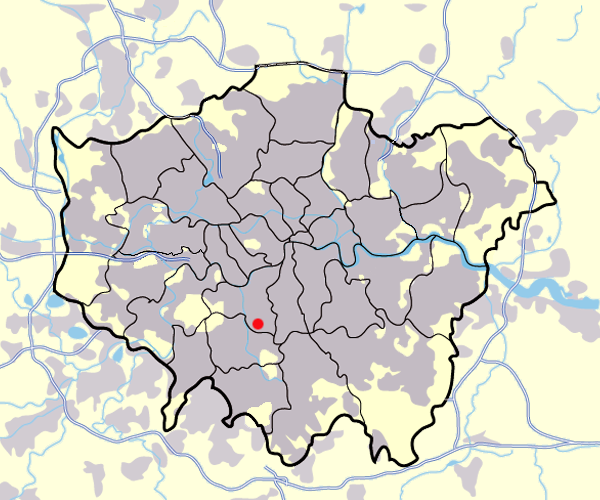
\includegraphics[width=.9\textwidth]{LondonMap}
\column{.5\linewidth}
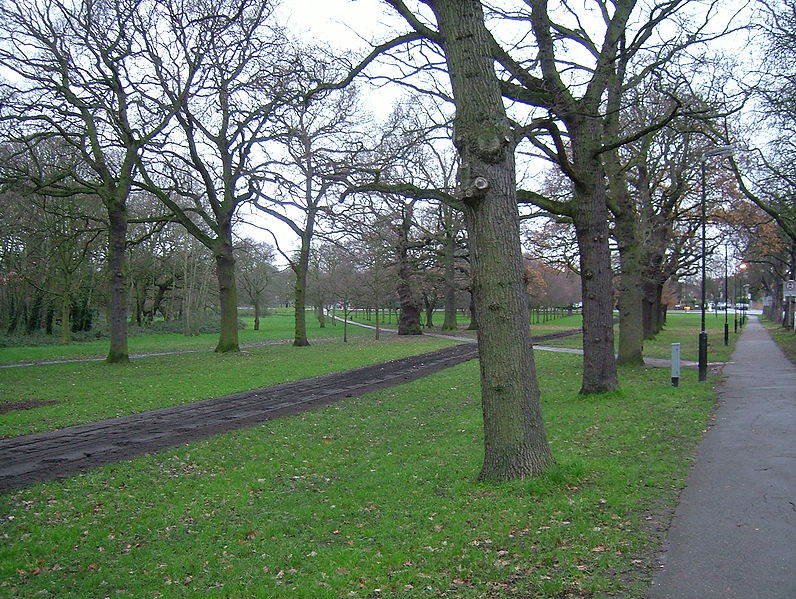
\includegraphics[width=.9\textwidth]{TootingBecCommon}
\end{columns}
\end{frame}

\begin{frame}{1987 --- Zambia, Africa}
\vspace{-1cm}
\begin{columns}[T]
\column{.5\linewidth}
\begin{center}
\only<1>{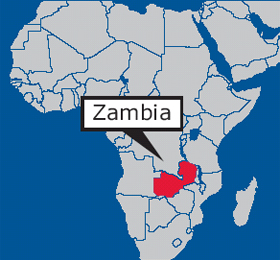
\includegraphics[width=.9\textwidth]{ZambiaMap}}
\only<2>{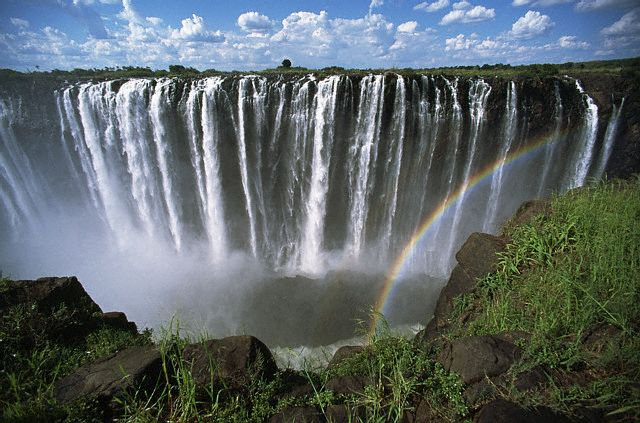
\includegraphics[width=.9\textwidth]{VictoriaFalls}\\
\vspace{.2cm}
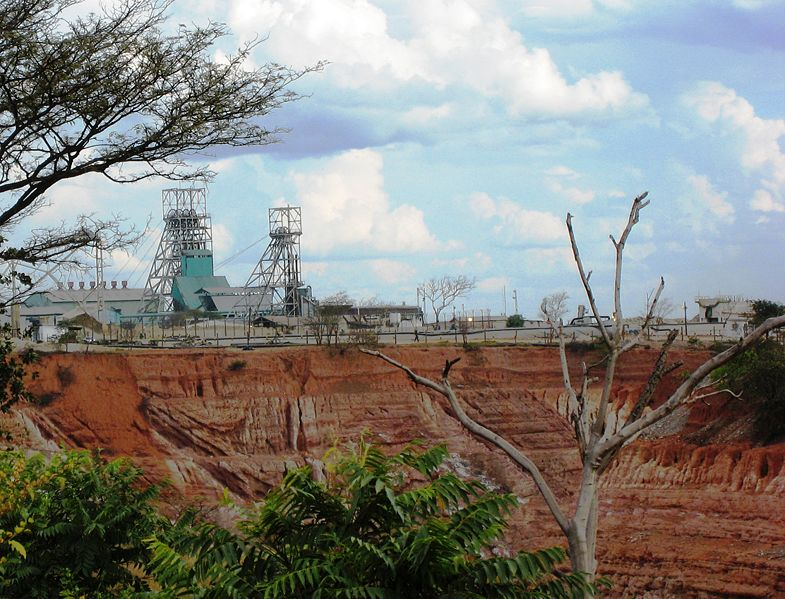
\includegraphics[width=.9\textwidth]{KitweCopperMine}}
\end{center}
\column{.5\linewidth}
\begin{center}
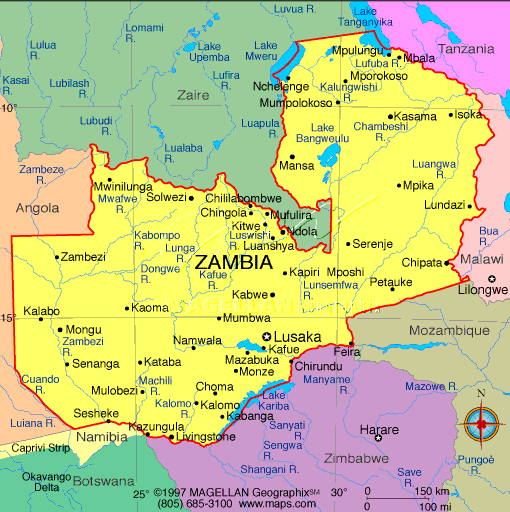
\includegraphics[width=.85\textwidth]{zambia}\\
\only<2>{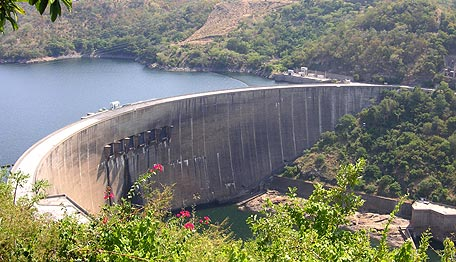
\includegraphics[width=.9\textwidth]{KaribaDam}}
\end{center}
\end{columns}
\end{frame}

\begin{frame}{1993 --- Back to England}
\begin{center}
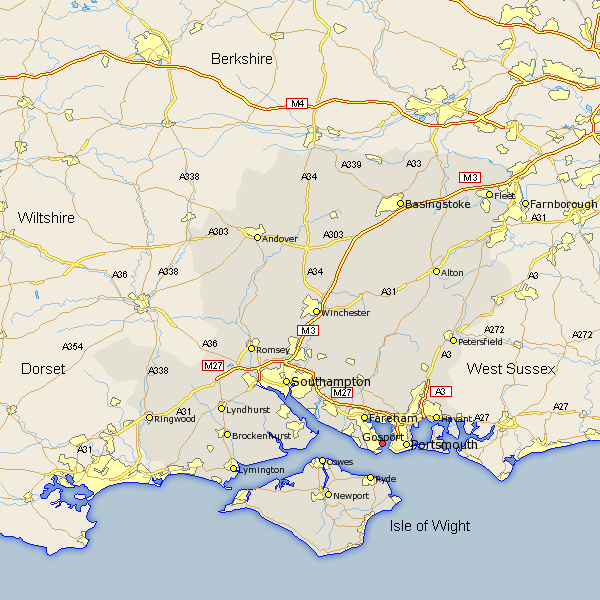
\includegraphics[height=.8\textheight]{GosportMap}
\end{center}
\end{frame}

\begin{frame}{2001 --- Oxford}
\begin{columns}[T]
\column{.35\linewidth}
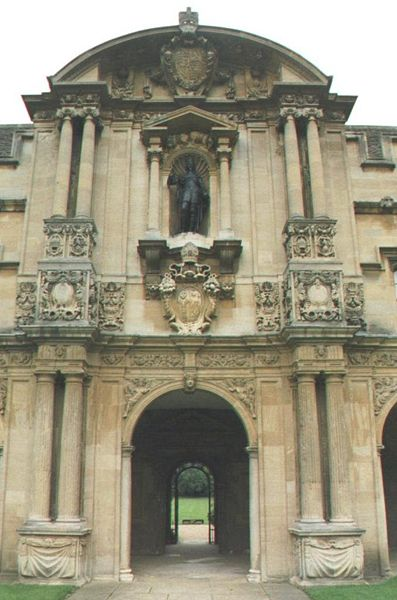
\includegraphics[width=.99\textwidth]{sjc1}
\column{.6\linewidth}
\hspace{.05\textwidth}
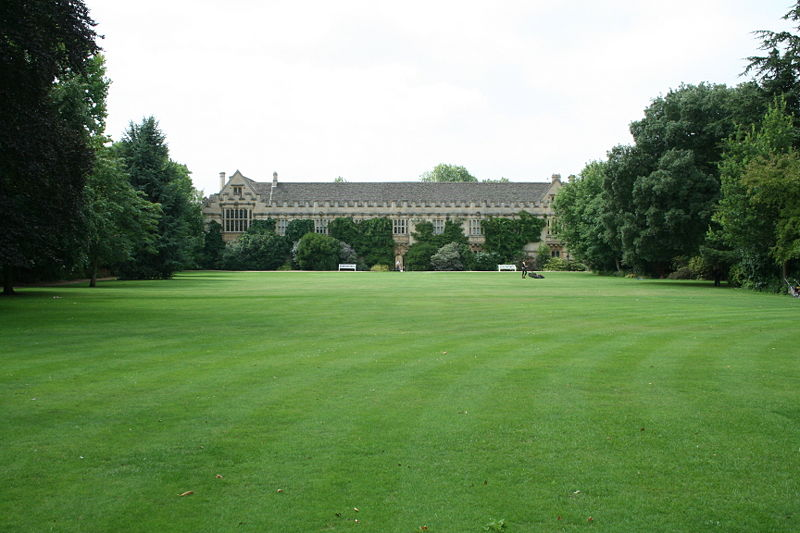
\includegraphics[width=.9\textwidth]{sjc2}
\begin{itemize}
\item 2001: BA, Mathematics \& Computer Science
\item 2004: DPhil, LSI DTC \& Computing Laboratory
\item 2008: Various postdocs
\end{itemize}
\end{columns}
\end{frame}

%%%%%%%%%%%%%%%%%%%%%%%%%%%%%%%%%%%%%%%%%%%%%%%%%%%%%%%%%%%%%%%%%%%%%%
\section{Introduction to functional curation}
%%%%%%%%%%%%%%%%%%%%%%%%%%%%%%%%%%%%%%%%%%%%%%%%%%%%%%%%%%%%%%%%%%%%%%
% * Explain problem, focus on sell, ability to describe and run a variety of experiments
% * Outline functional curation, demonstrate 2 example protocols

\begin{frame}{What is the problem?}
\begin{itemize}
\item Many (cardiac cell) models exist
  \begin{itemize}
  \item Multiple models of a system are developed to explore and compare hypotheses
  \item How do we choose between them?
  \end{itemize}
\item What functionality does a model have?
\item How do we robustly parameterise models and challenge them with data?
\item How can we determine a model's limitations or suitability for a given study?
\item When extending a model to explore a new experimental scenario, does it still reproduce the original behaviour?
\end{itemize}
\end{frame}

\begin{frame}{Models and experiments}
\begin{itemize}
\item We have languages (e.g.\ CellML) to describe mathematical models
\item Models are based on and tested by \alert{experiments}
\item We are developing
  \begin{itemize}
  \item A \alert{protocol language} to describe experiments
  \item A tool to run these on models and compare results
  \end{itemize}
\end{itemize}
\end{frame}

\begin{frame}{Potential applications}
\begin{itemize}
\item Rational model selection: based on ability to produce expected results for set of protocols
  \subitem{Or motivate further development if none can}
\item Explore which model features are essential for particular behaviours
\item ``Test-driven'' model development: continual comparison to set of protocols and experimental data
  \subitem{Build up a published library thereof}
\item Parameter fitting to a set of protocols
\item Parameter sweeps, sensitivity analysis, \ldots
\end{itemize}
\end{frame}

\begin{frame}{Example: S1-S2 restitution}
\begin{center}
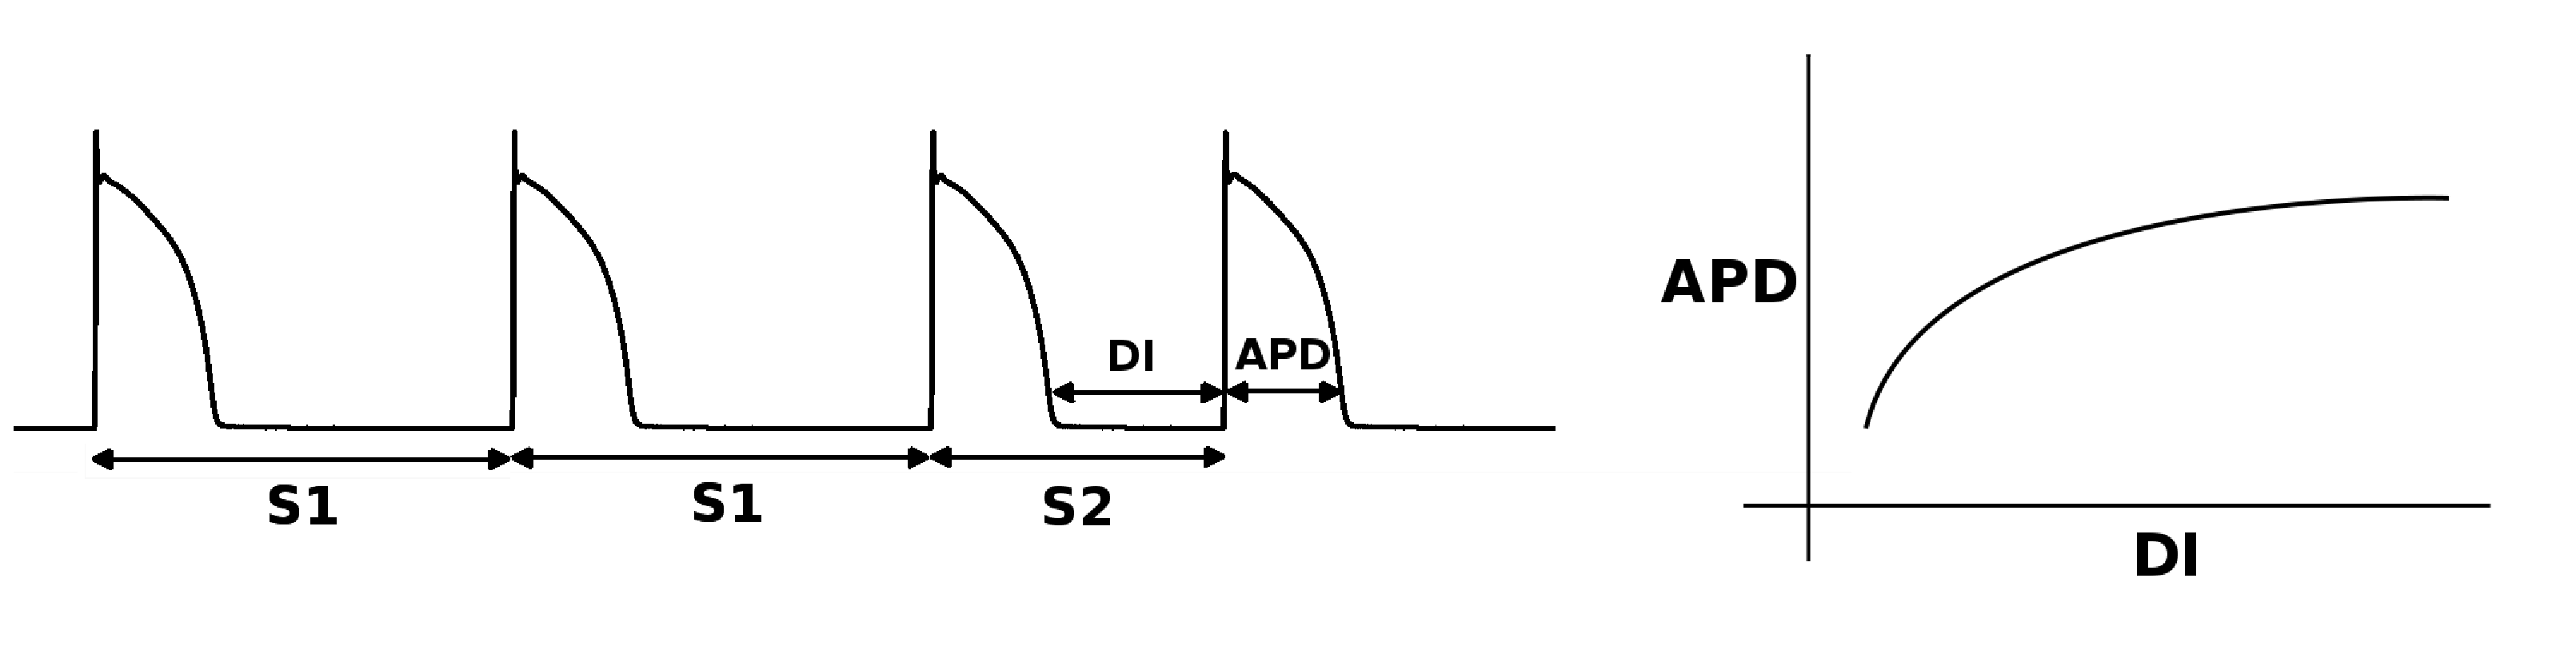
\includegraphics[width=\textwidth]{S1S2}
\end{center}
\end{frame}

\begin{frame}{Example: S1-S2 restitution on canine models}
TODO: update figures from latest code
\begin{columns}[T]
\begin{column}{.33\linewidth}
\begin{center}
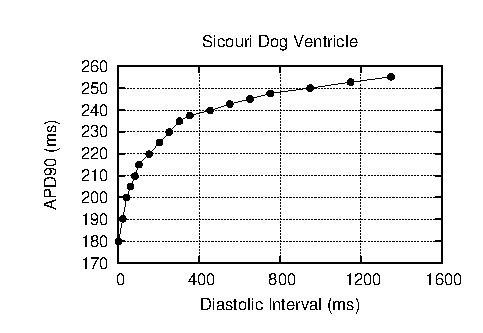
\includegraphics[width=\textwidth]{sicouri_dog_ventricle_s1s2_curve}\\
\vspace{.1cm}
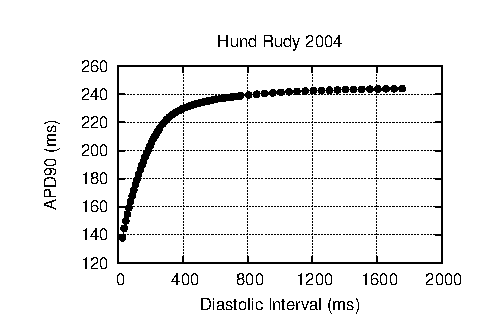
\includegraphics[width=\textwidth]{hund_rudy_2004_s1s2_curve}
\end{center}
\end{column}
\begin{column}{.33\linewidth}
\begin{center}
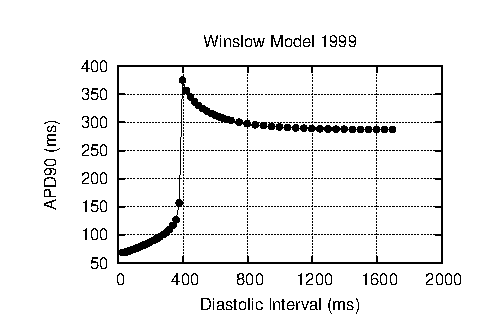
\includegraphics[width=\textwidth]{winslow_model_1999_s1s2_curve}\\
\vspace{.1cm}
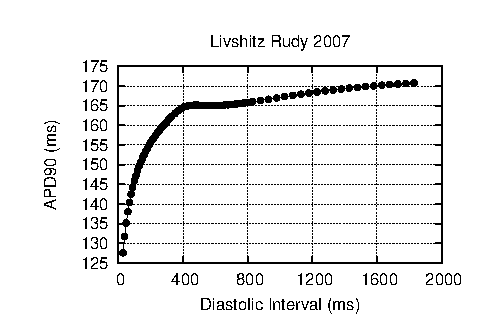
\includegraphics[width=\textwidth]{livshitz_rudy_2007_s1s2_curve}
\end{center}
\end{column}
\begin{column}{.33\linewidth}
\begin{center}
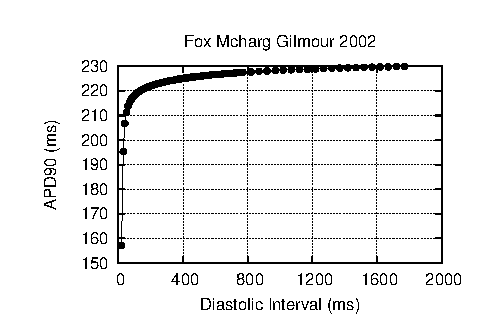
\includegraphics[width=\textwidth]{fox_mcharg_gilmour_2002_s1s2_curve}\\
\vspace{.1cm}
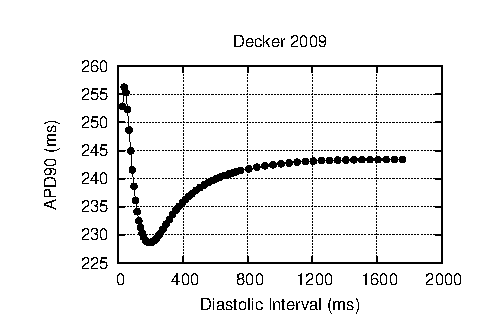
\includegraphics[width=\textwidth]{decker_2009_s1s2_curve}
\end{center}
\end{column}
\end{columns}
\end{frame}

\begin{frame}{Example: S1-S2 restitution on human models}
TODO: update figures from latest code
\begin{columns}[T]
\begin{column}{.33\linewidth}
\begin{center}
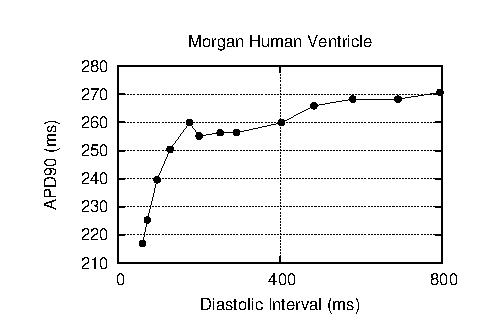
\includegraphics[width=\textwidth]{morgan_human_ventricle_s1s2_curve}\\
\vspace{.1cm}
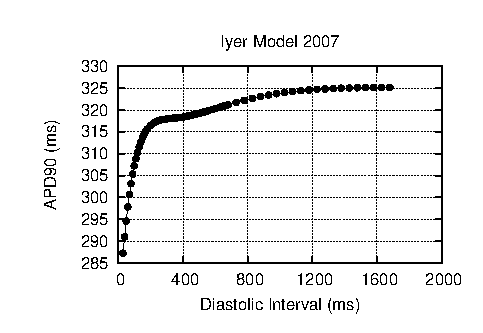
\includegraphics[width=\textwidth]{iyer_model_2007_s1s2_curve}
\end{center}
\end{column}
\begin{column}{.33\linewidth}
\begin{center}
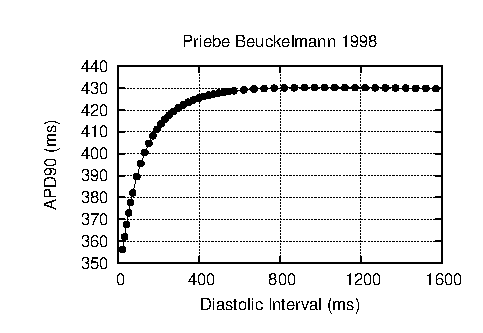
\includegraphics[width=\textwidth]{priebe_beuckelmann_1998_s1s2_curve}\\
\vspace{.1cm}
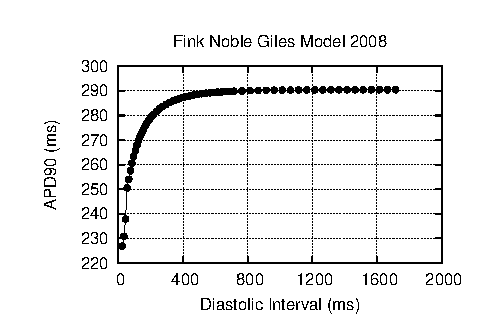
\includegraphics[width=\textwidth]{fink_noble_giles_model_2008_s1s2_curve}
\end{center}
\end{column}
\begin{column}{.33\linewidth}
\begin{center}
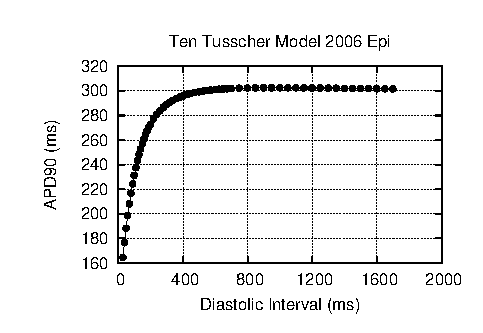
\includegraphics[width=\textwidth]{ten_tusscher_model_2006_epi_s1s2_curve}\\
\vspace{.1cm}
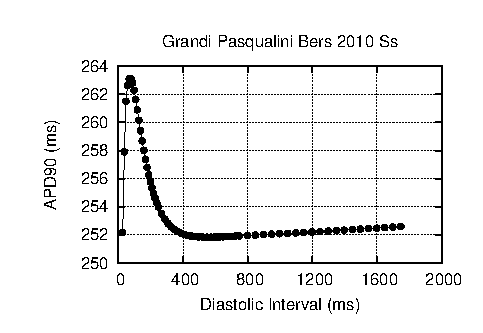
\includegraphics[width=\textwidth]{grandi_pasqualini_bers_2010_ss_s1s2_curve}
\end{center}
\end{column}
\end{columns}
\end{frame}

\begin{frame}{Example: $I_{\textrm{Ca}_L}$ voltage clamp}
\begin{center}
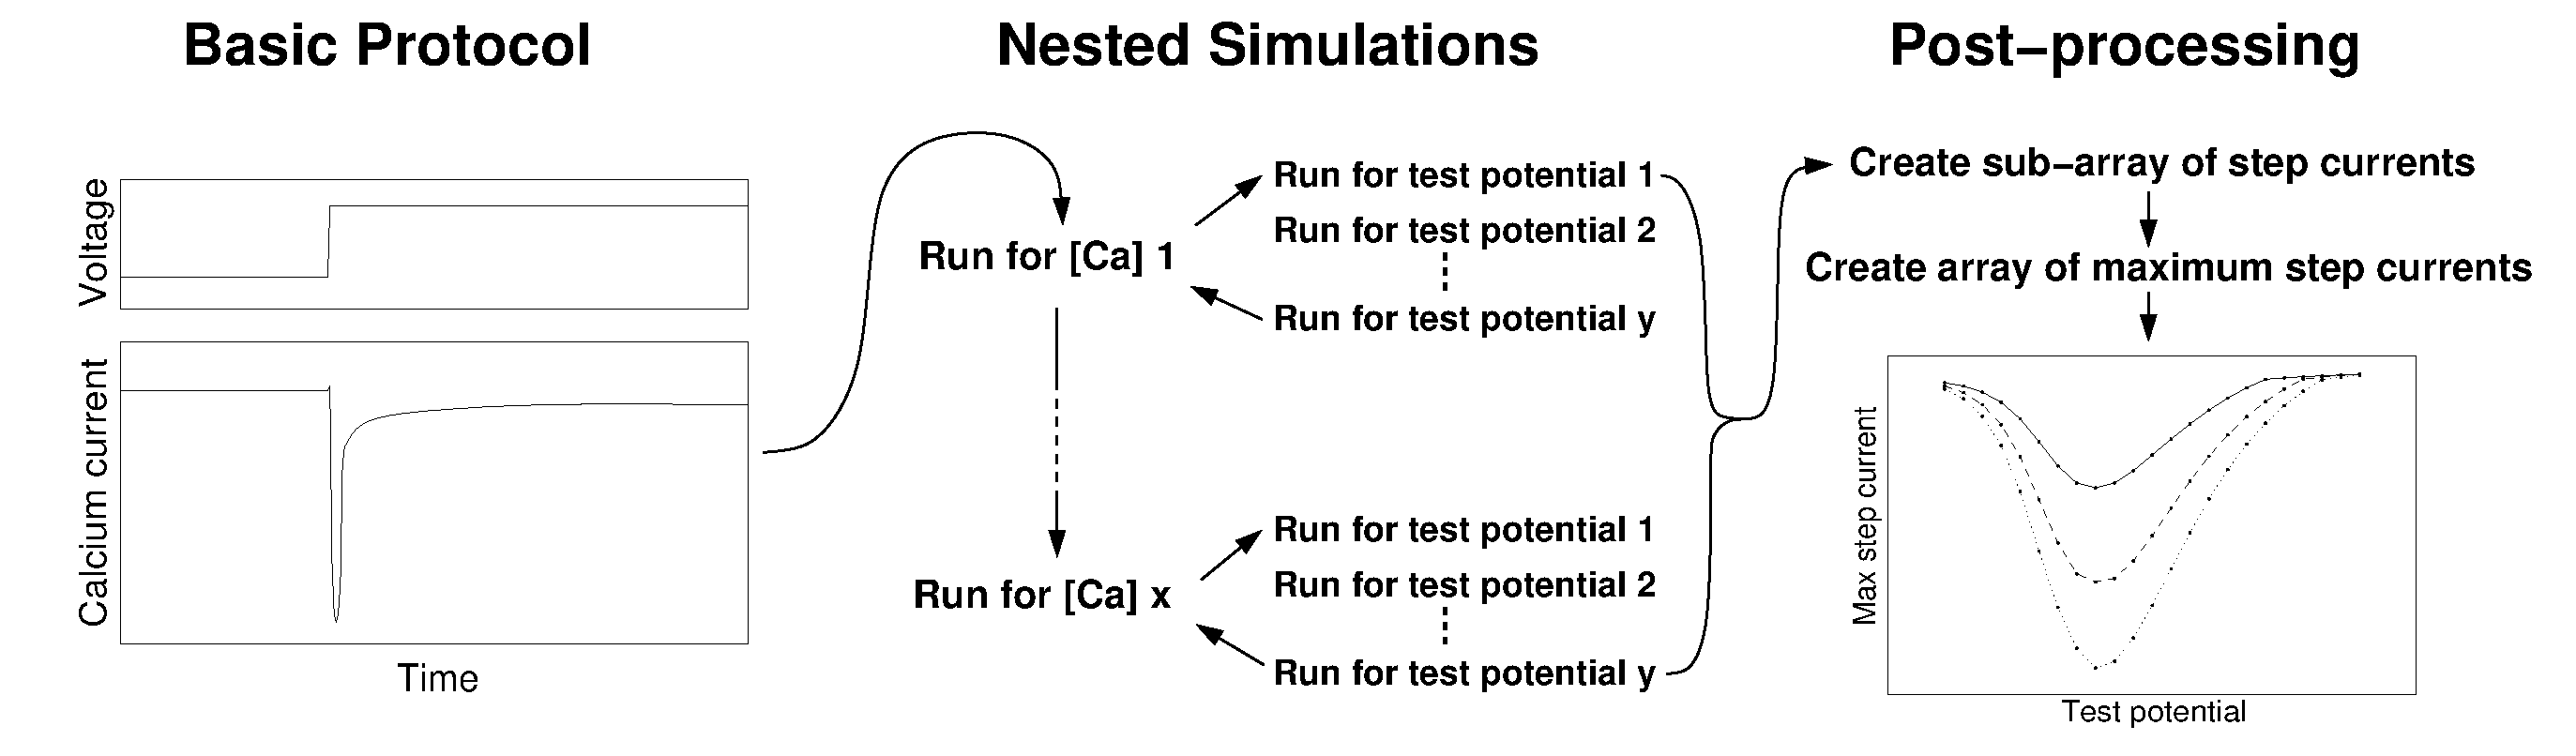
\includegraphics[width=\textwidth]{ICaLIntro}
\end{center}
\end{frame}

\begin{frame}{Example: $I_{\textrm{Ca}_L}$ voltage clamp}
Any suggestions for nice models to show?
\end{frame}

%%%%%%%%%%%%%%%%%%%%%%%%%%%%%%%%%%%%%%%%%%%%%%%%%%%%%%%%%%%%%%%%%%%%%%
\section{Protocol language details}
%%%%%%%%%%%%%%%%%%%%%%%%%%%%%%%%%%%%%%%%%%%%%%%%%%%%%%%%%%%%%%%%%%%%%%

\begin{frame}{Notes}
 * Further details on features, emphasis on what other kinds of protocol can be represented
 * Use flowcharts sent to Dave
 * Have a `describe your favourite protocol' challenge
 * Use some stuff from COMBINE talk: model interface, seq and nest sims, post-proc, libraries
\end{frame}

\begin{frame}{Technical challenges}% From DTC proj talk
\begin{itemize}
\item Dealing with variations in modelling conventions
  \begin{itemize}
  \item Need to run the same protocol on any model
    \subitem{e.g.\ variations in naming $\rightarrow$ annotation with \alert{ontologies}}
  \item Need to be able to compare models coherently
    \subitem{e.g.\ units conversions}
  \end{itemize}
\item Expressivity vs simplicity for the protocol language
  \begin{itemize}
  \item both for inputs
  \item and post-processing
  \end{itemize}
\end{itemize}
\end{frame}

\begin{frame}{Interfacing protocols and models}
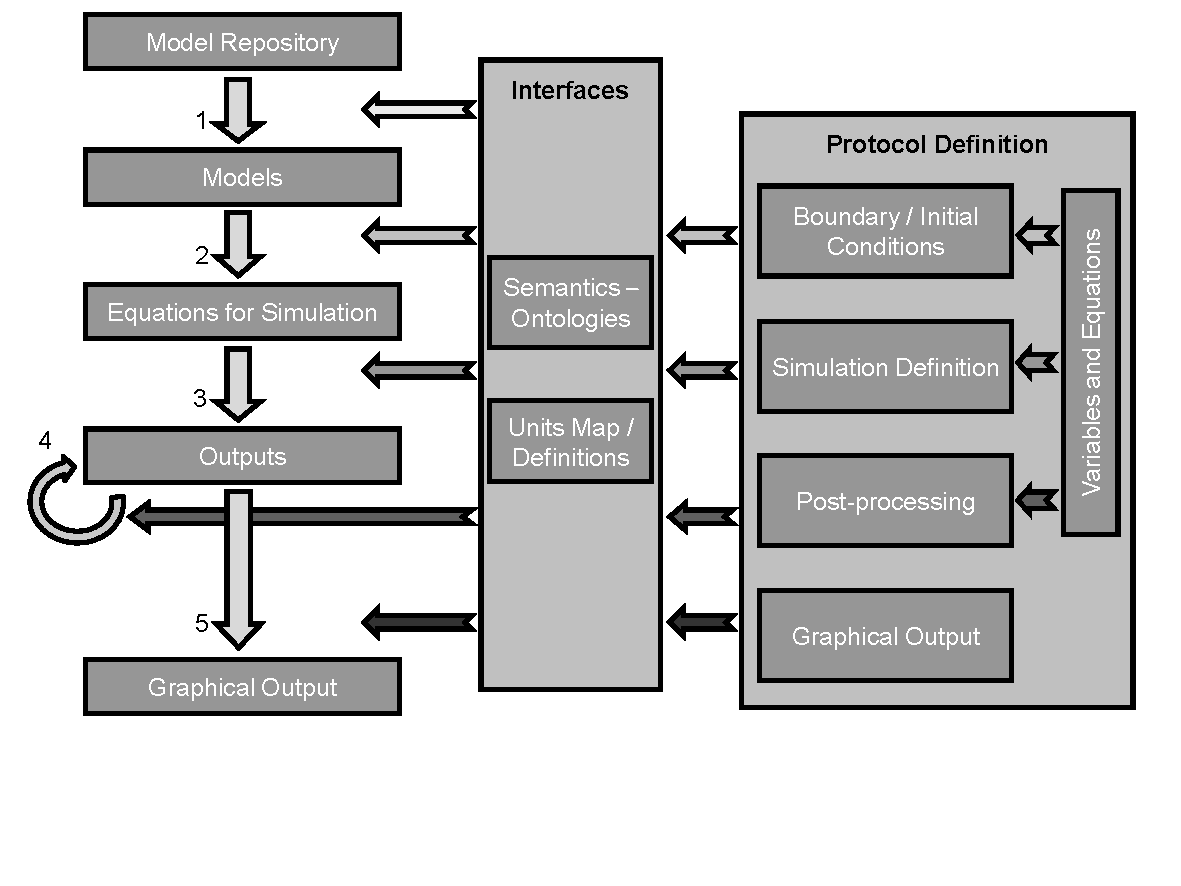
\includegraphics[width=.9\textwidth]{schematic_v4}
\end{frame}

%%%%%%%%%%%%%%%%%%%%%%%%%%%%%%%%%%%%%%%%%%%%%%%%%%%%%%%%%%%%%%%%%%%%%%
\section{Conclusions and future directions}
%%%%%%%%%%%%%%%%%%%%%%%%%%%%%%%%%%%%%%%%%%%%%%%%%%%%%%%%%%%%%%%%%%%%%%

\begin{frame}{}
 * Caveats: usability, performance, still prototype; but lots of scope!
 * Conclusions and plans
\end{frame}

%%%%%%%%%%%%%%%%%%%%%%%%%%%%%%%%%%%%%%%%%%%%%%%%%%%%%%%%%%%%%%%%%%%%%%
\begin{frame}{Acknowledgments}
Gary Mirams, Chaste team, Alan Garny, Steven Niederer

\begin{center}

\includegraphics[scale=.9]{chaste-266x60}\\ \vspace{.4cm}

\includegraphics[width=.55\textwidth]{EPSRC1RGBLO} \hspace{.1cm}

\includegraphics[scale=.55]{logo_msr}
\end{center}
\end{frame}

\end{document}
